\subsection{Introduction}
Generally, it can be affirmed that different parts of the brain are responsible
for different actions as well as respond to different sensory inputs. It is
thought to be the most complex organ of the body, moreover it consumes more or less
\(20\%\) of the overall ATP produced. The cortex is made of approximately \(14-16\)
billions neurons, even if it is not a homogeneous tissue, as it is made of various
layers with different properties. The cortex neurons form about \(20\) trillions
synapses. In addition, pyramidal cells (a particular type of neurons) are the
most common excitatory cells, exhibiting the longest axons and big cell bodies.
It is important to point out that the brain is highly redundant, as a matter of fact
just few regions are highly specialized, making easier to recover from injuries
due to brain plasticity.\\
The brain can be studied at several distinct scales, according to the recording site
and the number of recorded neurons producing a certain electrical signal. In general,
it can be stated that different neurons will respond to stimuli in different ways.\\
The Local Field Potential (LFP) refers to the electric potential measured in the
extracellular space around neurons. Notice that it requires invasive electrodes
implanted into the subject brain, thus it has nothing to do with EEG. If compared to
spike recording, here the electrode is not inside or extremely close to a single neuron,
therefore the signal travels through the extracellular space according to Maxwell's
equations. The \textit{local} term is misleading, as it is meant to indicate that
the LFP is derived from a small number of sources: the action potential fired by a
neuron is highly attenuated by the extracellular space, thus the electrode can record
potentials in a limited radius. Nonetheless, the LFP signal still displays a fair
signal-to-noise ratio (SNR). Spiking activity and Local Field Potential are closely
related to one another, as they influence each other, however it is crucial to point
out that they are not exactly the same signal, just observed at different scales.
LFP carries information not present in the spiking activity and vice-versa.
\subsection{LFP Recording Techniques}
The \textit{in vivo} Local Field Potential signal is mainly recorded by exploiting
two techniques:
\begin{itemize}
    \item \textbf{Electrocorticography (ECoG):} subdural grids are placed directly on
    the top of the cortex, under the dura matter), resulting in a significantly
    invasive implant.
    \item \textbf{Stereo Electroencephalography (SEEG):} linear multi-electrode shafts
    are directly implanted into the grey matter, thus the invasiveness is reduced,
    as only small holes on the skull are necessary to insert the long linear electrodes.
\end{itemize}
As said above, the cortex is structured in multiple layers, each with its own
properties, such as the density of neurons. Generally, deeper layers' neurons
tend to project axons towards the surface, while upper layers' cells project axons
mostly horizontally. As a result, the recorded activity is greatly variable according
to the selected recording site, as depicted below. In addition, notice that also the
SNR is highly influenced by the location of the recording site, since it increses
with the distance from the source.
\begin{figure}[H]
    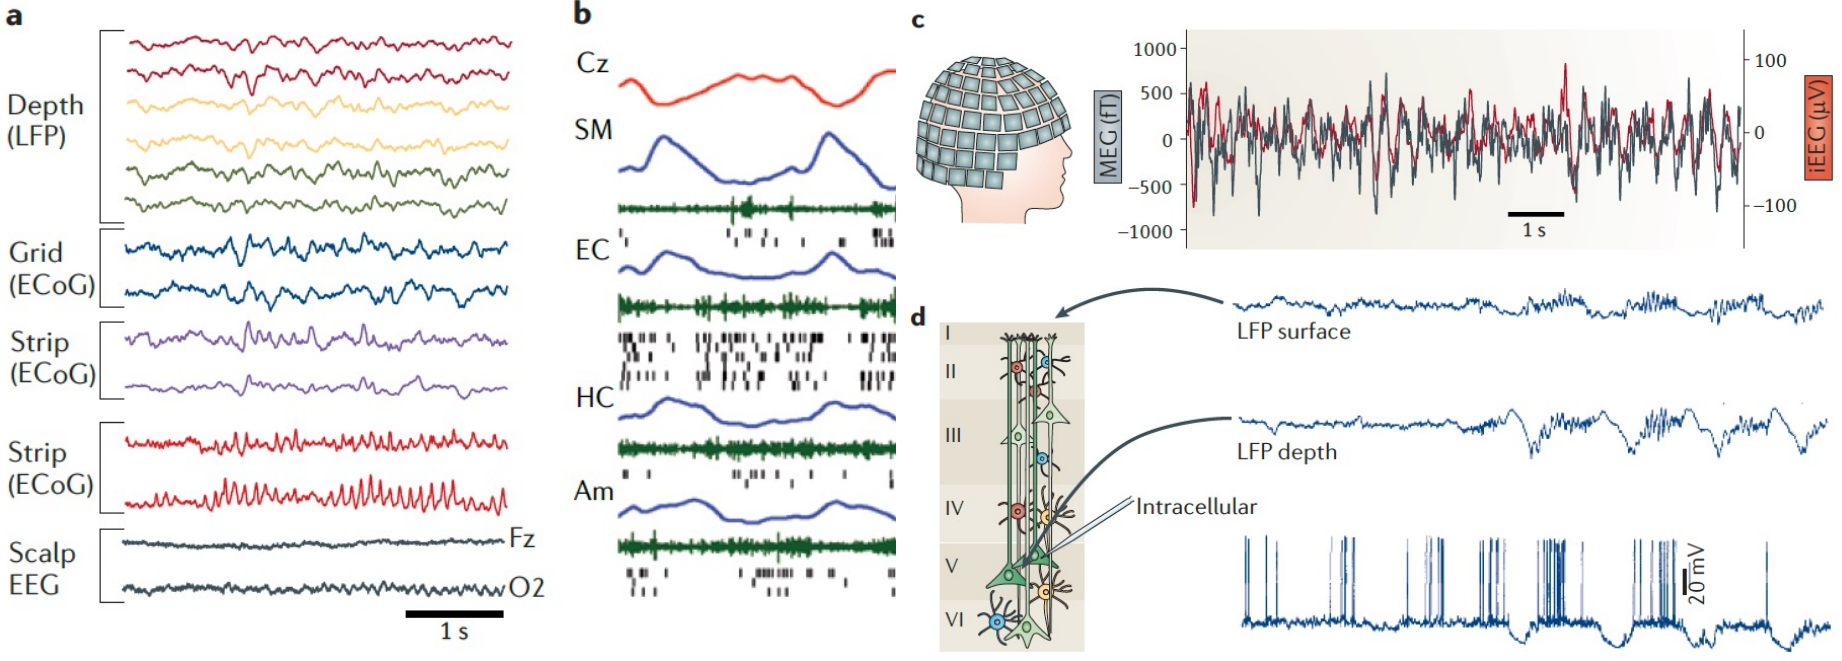
\includegraphics[scale=0.45]{9_1}
    \centering
\end{figure}
\subsection{LFP Signal Components}
In order to understand the meaning of the Local Field Potential, it is fundamental to
understand which are the factors contributing to it. The extracellular field is
a superimposition of:
\begin{itemize}
    \item Any excitable membrane (such as axons), always trying to balance the inner
    and outer ions concentrations, generating electrical currents.
    \item Synaptic activity between cells, generating the largest extracellular
    currents.
    \item Fast action potentials, where Na\({}^+\) ions contributes to high frequency
    activity.
    \item Calcium spikes, recorded by exploiting calcium imaging techniques.
    \item Intrinsic currents and resonances, giving birth to membrane responses.
    \item Spikes after hyperpolarization.
    \item \dots
\end{itemize}
In general, it can be said that the surrounding activity of neurons highly affects the
LFP by influencing the transmembrane potential of cells.
\begin{figure}[H]
    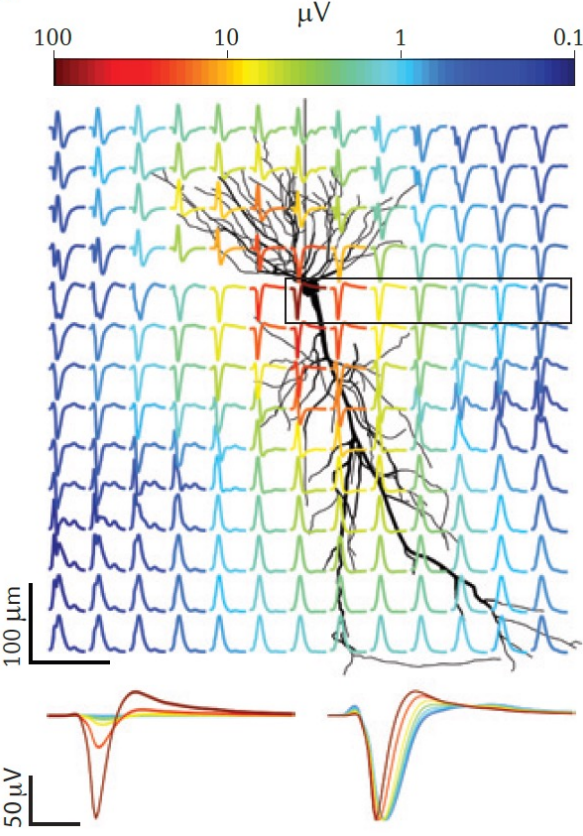
\includegraphics[scale=0.42]{9_2}
    \centering
\end{figure}
Also the neuronal geometry as well as the architecture has a huge impact on the
recorded LFP signal. In particular, nerons can be roughly divided into two main
classes: linear and spherical (often called stellate). The shape of a neuron highly
influence the way the electrical signal travels and propagates in the extracellular
field. Pyramidal neurons, which are considered to belong to the linear class, are
characterized by a significant distance between soma and apical dendrites, generating
large dipoles, thus resulting in a strong field. On the contrary, spherical neurons
tend to emanate dendrites of approximately equal size in all directions, implying
almost no separation between sink and source, with a small contribution to the overall
electrical field, as signals cancel out each other.
\begin{figure}[H]
    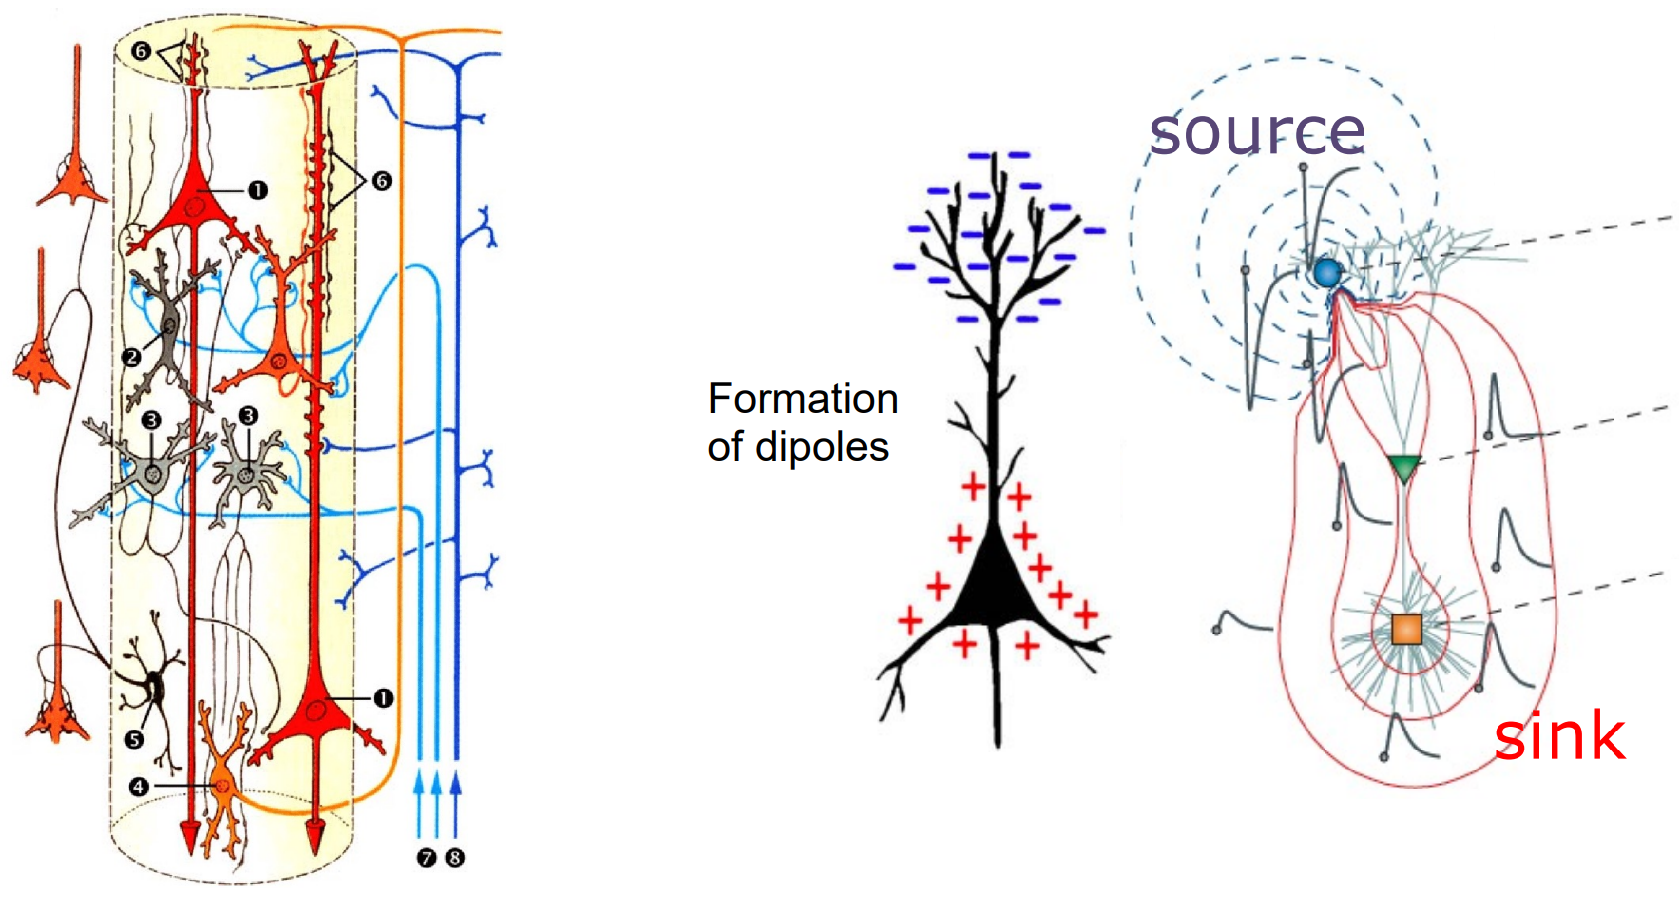
\includegraphics[scale=0.42]{9_3}
    \centering
\end{figure}
A further factor affecting the LFP signal is the temporal scaling. A temporal
superimposition of a large number of activated neurons will increase the LFP
signal: this phenomenon is known as synchronization. The so-called \textit{Beta rhythm}
is a peculiar type of synchronization occurring in reaching and motion tasks, but this
synchronization is suppressed as soon as the reaching movement is completed. Another
important feature of temporal scaling is the \(\frac{1}{f^{\alpha}}\) frequency decay:
the amplitude of the signal exhibits a power law decay towards high frequencies. This
may be partially explained by the low-pass filtering performed by dendrites.

\subsection{The Forward Problem}
By assuming a homogeneous and isotropic conductivity, it is possible to easily
solve the so-called \textit{forward problem} by exploiting the Maxwell's equations.
The \textit{forward problem} consists to reconstruct the measured eletrical field
- i.e. the LFP - by knowning the sources which generated it. Unluckily, the
brain conductivity is neither homogeneous nor isotrpic and this generates several
problems when studying how the eletrical signal propagates through the nerual tissue,
this phenomenon is thus denominated volume conduction. Generally, when analyzing a
neural signal, it is believed that coherent activity reflects functionally relevant
processing; however, volume conductivity represents a significant issue, as it
tends to amplify this, leading to an overestimation of the coherent activity
in brain.\\
More in detail, the \textit{forward problem} indicates the modelling of the system
responsible for the generation of a given recorded signal. It is opposed to the
\textit{inverse problem}, consisting in sources localization. A possible approach
to the \textit{forward problem} is by exploiting compartimental models, then
properly tuning the model parameters. Although this approach looks promising,
it is computationally costly. On the other hand, single-compartment models
are too simplistic to properly describe the structure of a neuron.\\
When trying to address the \textit{forward problem} it is important to recall
that the synaptic connectivity highly affects the LFP. On one side, it
determines the spike train statistics (the so-called temporal coding), creating
correlation patterns for the synaptic inputs. On the other side, the spatial
distribution of synapses highly affects how inputs are translated into LFP.
To sum up, it is not just a single neuron geometry that determines the LFP
dynamics, but also the network spatial distribution: at the micro and meso
scales the structure of the network plays a crucial role in determining
the function.

\subsection{Functional Decomposition}
The Local Field Potential, as well as other signals such as EEG and MEG ones,
is usually decomposed into several frequency bands thanks to filtering.
These bands are often referred to as Berger bands, even if they are far from
being accurate between different subjects and even within the same subject in
different time instants. Usually, three main groups are determing by looking
at the correlation between two signals as a function of their frequency.
These three clusters are:
\begin{itemize}
    \item Slow rhythms with a high oscillatory activity: \(0\sim{50}\,Hz\)
    \item Gamma oscillations mediated by rhythmic inhibition: \(<100\,Hz\)
    \item High gamma activity, reflecting the Multi Unit Activity (MUA) close
    to the electrode, proportional to the real spiking activity: \(100\sim{150}\,Hz\)
\end{itemize}
\begin{figure}[H]
    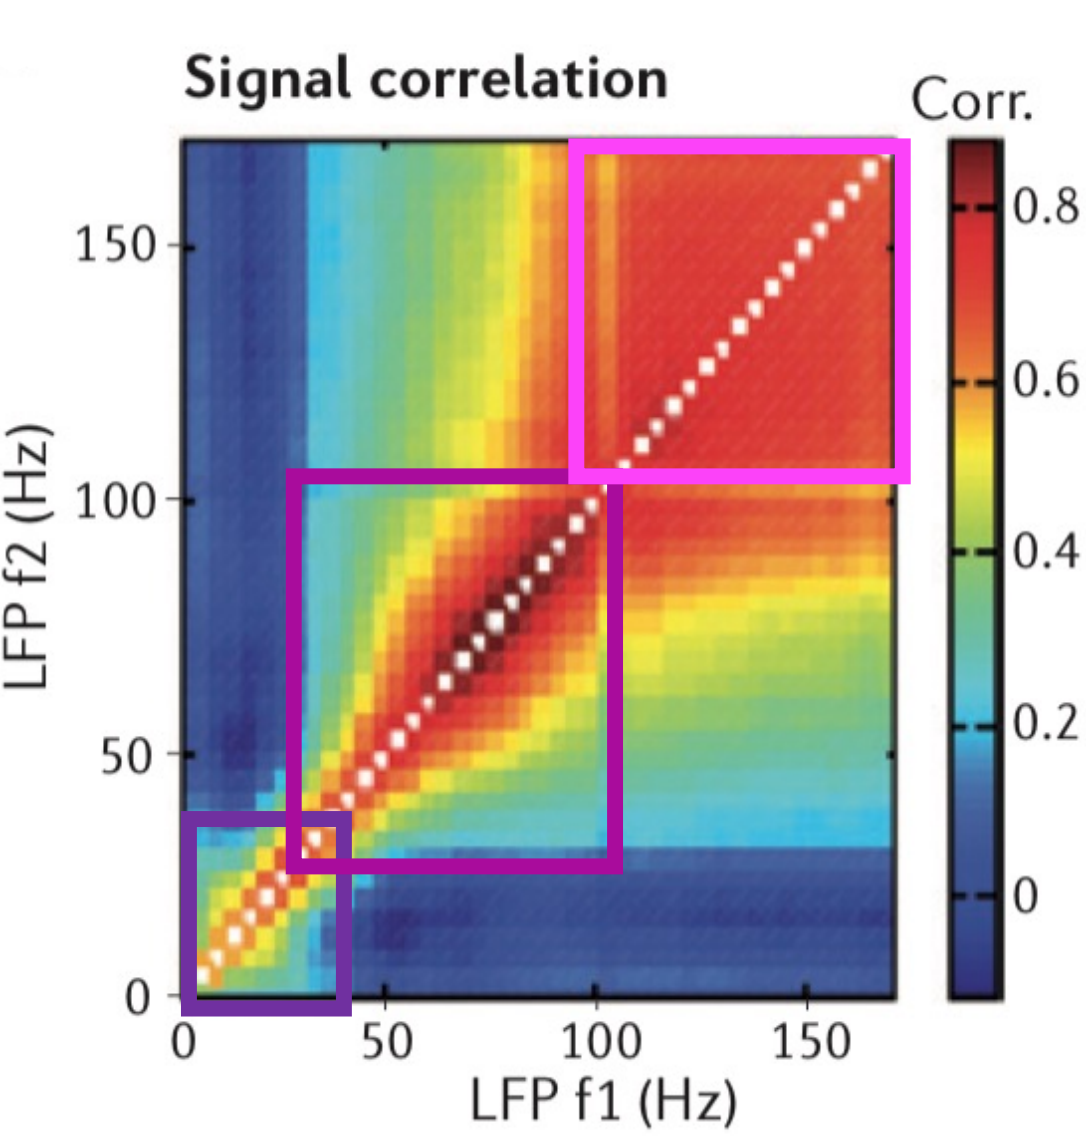
\includegraphics[scale=0.35]{9_4}
    \centering
\end{figure}